\chapter{Experiments}
The main purpose of this chapter is to compare animations generated using IK
with baked animations. The comparison is broken up into two categories - visual
quality and performance. 

\section{Baked animations}
 In order to conduct the experiments, a second set of animations were created
 for each of the examples which are shown in the demo application. Below is an
 explanation of the process of creating this second set of animations. \\

\noindent\textit{Spider}

The baked animation version of the spider was animated in Blender. The model
has both idle and walking animations which, in Blender, are placed on
a single timeline, one after the other, as shown in Fig. \ref{fig:timeline}.
Once the model is imported into Unity, the animations can be broken up into
their separate cases, as shown earlier in Chapter 3.3.1 (Fig.
\ref{fig:anim_chunk}). 

\begin{figure}[h!]
    \centering
    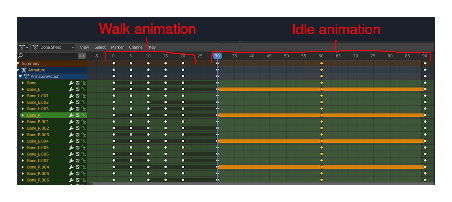
\includegraphics[width=0.7\textwidth]{grafika/blender_timeline.eps}
    \caption{Two animations on a single timeline}
    \label{fig:timeline}
\end{figure}

Once the animations have been imported, a new animation controller is created
for the new spider. The animations are added, this time with the use of a blend
tree (Fig. \ref{fig:s_blendtree}) to, as the name suggests, blend between the
animation smoothly. A third animation state is added to the blend tree
which is the equivalent of the walking animation, but the animation speed is set
to a negative value. This plays the animation in reverse and is used when the
spider is walking backwards. 

\begin{figure}[h!]
    \centering
    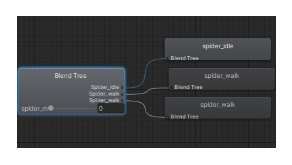
\includegraphics[width=0.7\textwidth]{grafika/spider_blend.eps}
    \caption{Blend tree containing animations for the spider}
    \label{fig:s_blendtree}
\end{figure}

A variable named \textit{spider\_movement} is created in order to control the
animations that are to be played in a given situation, and the manner in which
the transitions should be blended. The thresholds for each animation can be
defined in the blend tree's configuration in the animator (Fig. \ref{fig:s_blendconf}).

\begin{figure}[h!]
    \centering
    \captionsetup{justification=centering}
    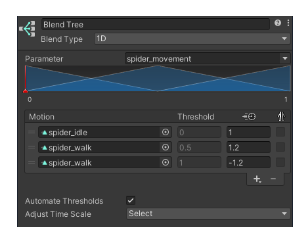
\includegraphics[width=0.7\textwidth]{grafika/spider_blendconf.eps}
    \caption{Configuration of the spider's blend tree which is dependent on
    the \textit{spider\_movement} variable}
    \label{fig:s_blendconf}
\end{figure}

In the spiders movement script, this variable can then be set in reaction to
certain inputs so that the proper animation is activated for each given situation.
To achieve the transition blending, the \textit{spider\_movement} variable
should not be set outright to the value which corresponds to the next animation
state. Instead, the \textit{\_animator.SetFloat} method is used, where the
\textit{\_animator} is a reference to the spider's Animator component. This
method allows the value of \textit{spider\_movement} to be interpolated from the value of
the current animation state to another desired value.
\newline
\begin{lstlisting}[basicstyle=\footnotesize, numbers=none,frame=single,
caption={Transitioning to the spider's idle animation using the
\textit{SetFloat} method},captionpos=b, label=stretch, language={[Sharp]c}]
    if (verticalAxis == 0f && horizontalAxis == 0f)
        _animator.SetFloat("spider_movement", 0f, 0.05f, Time.deltaTime);
\end{lstlisting}

This version of the spider has its movement inspired by the spider from the game
Minecraft, which means that its rotation on the x and z axes is locked. The
spider can rotate about the y-axis when turning to face a different direction,
but it will not adjust to variations in the surface which it walks upon.
Additionally, when the spider encounters a wall, it begins moving
vertically instead of horizontally until it scales the entire obstacle.

\subsubsection{Human}
The baked version of the human character, which performs an animation sequence
consisting of pressing buttons, is animated in Blender. The animation plays one
full sequence of pressing a single button. Chunks of the same animation are used
in the IK version of this animation sequence, described in the previous chapter,
but the baked animation uses the full animation while the IK version uses only
the beginning and the end. However, the animation is still broken up into three
parts when imported into Unity: the raising of the hand, the button pressing
motion, and the lowering of the hand (Fig. \ref{fig:bp_clips}). This is done
because when the character is pressing multiple buttons in a row, the hand
should not be lowered to its starting position after every press.

\begin{figure}[h!]
    \centering
    \captionsetup{justification=centering}
    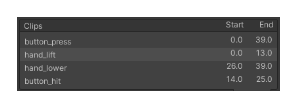
\includegraphics[width=0.7\textwidth]{grafika/bp_clips.eps}
    \caption{The full button press animation is broken up into 3 separate clips}
    \label{fig:bp_clips}
\end{figure}

Another animation controller is created for this version of the human. Unlike
the spider example, the animation states do not have to be blended as they are
all clips which combine to create the full button press animation, and the
transitions are seamless as they are. Because of this, the animation states for
the three animation clips are not part of a blend tree, and instead are just
"floating" states with no defined transitions. The logic for which animation
should be played at what time is defined in the main script attached to the
character. 

The script is a simplified version of the one which controls the IK version of
this character's animation. It has no need for the public parameters present in
it's IK version because there is no IK rig, IK target, or button transforms
which it needs to control. Due to this, there is no list containing the sequence
of buttons to be pressed. It is instead replaced by an integer value which
dictates the number of button presses to execute in one animation sequence in
order to convey the idea that the character is pressing multiple buttons in
a sequence. 

As with the IK version of this script, the logic is based on a set of coroutines
which control the flow of the animation sequence. However, only the
\textit{HandAnimation} coroutine is used as a building block for the sequence
because the whole action is now constructed using baked animations. When the
script receives an input and the animation is not already playing, the sequence
begins by setting the \textit{idle} variable to false in order to prevent the sequence
from being repeated while it is still in progress. All required animation clips
are then set off one after the other, starting with the animation to lift the
hand. This is then followed by the animation clip which is responsible for
hitting the button, and it is repeated in a loop for the number of times defined
by the button press count parameter. Finally, the animation clip for lowering
the hand is executed, and the \textit{idle} boolean is set to true before
terminating the sequence.

\section{Visual Comparison}
The goal of using inverse kinematics to procedurally animate a model in video
games is to achieve a more natural interaction between a character and the
environment. The realism of the interaction is conveyed through how it looks,
and how the animation is a more realistic representation of how such an action
might look in real life. Therefore, the visual integrity of the IK animation as
it adapts to a plethora of scenarios is what sets it apart from a classic
approach through baked animations. 

The walking animation, or any basic movement animation, is the core of what
most characters will be displaying a majority of the time. That being the case,
a natural movement animation will contribute the most to the overall look and
feel of the character. This difference can be clearly noticed by comparing the
two version of the spider implemented in the demo application created for the
purpose of this paper. 

Starting with the idle position, both models look quite natural standing on
a flat surface, as seen in Fig. \ref{fig:sp_flat}.

However, this changes when the surface is uneven. The IK acting on
the legs of the spider on the right in Fig. \ref{fig:sp_round} is able to use
its ray casts to match the surface exactly, while the baked version of the
spider (left) doesn't have this mechanism, and its legs can be seen floating in
the air. The same effect is observed when the spider is moving. The baked
version's legs float when it is moving over uneven or slanted surfaces, which
makes it seem as if the spider was swimming through the air. 

Another difference between the two spiders is how they climb walls. Whereas the
IK version is able to treat it the same as any other surface, the baked version
keeps does not adjust its rotation, and instead climbs the wall head on (Fig.
\ref{fig:sp_wall}). This kind of rotation could have been implemented, however,
the transition between floor and wall would be very unnatural either way and so
an implementation inspired by the spiders in the game Minecraft was used
instead.

\begin{figure}[!h]
    \centering
    \captionsetup{justification=centering}
    \begin{subfigure}{\textwidth}
        \centering
        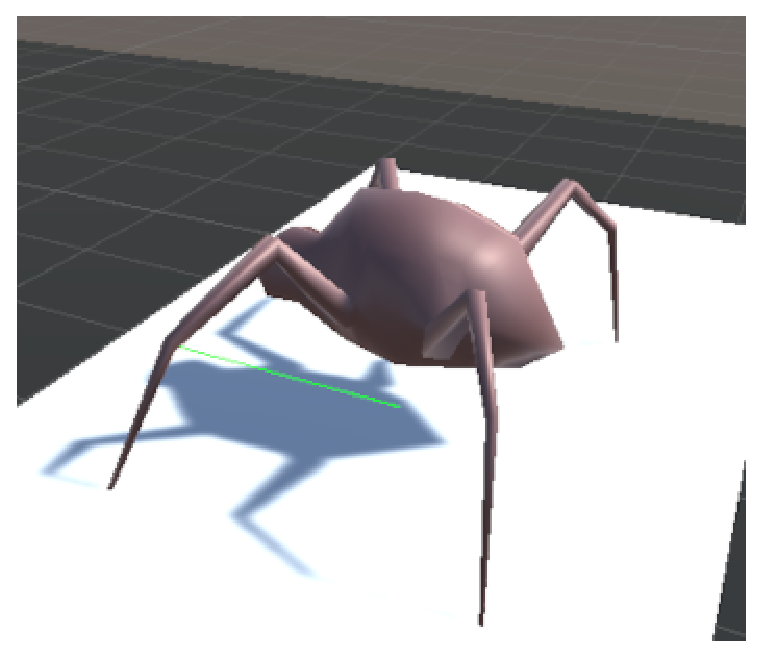
\includegraphics[width=0.4\linewidth]{grafika/sp_b_flat.eps}
        \hspace{0.1cm}
        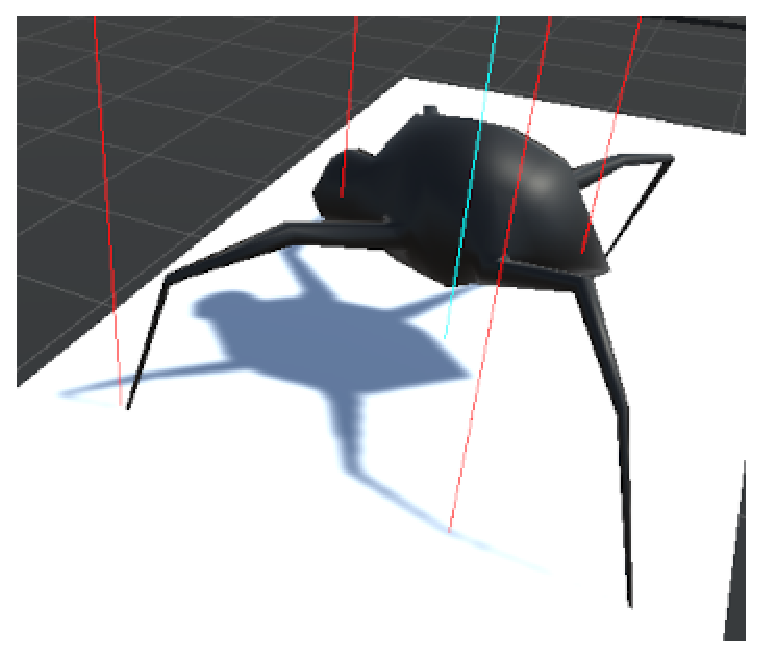
\includegraphics[width=0.4\linewidth]{grafika/sp_ik_flat.eps}
        \subcaption{}
        \label{fig:sp_flat}
    \end{subfigure}
    \begin{subfigure}{\textwidth}
        \centering
        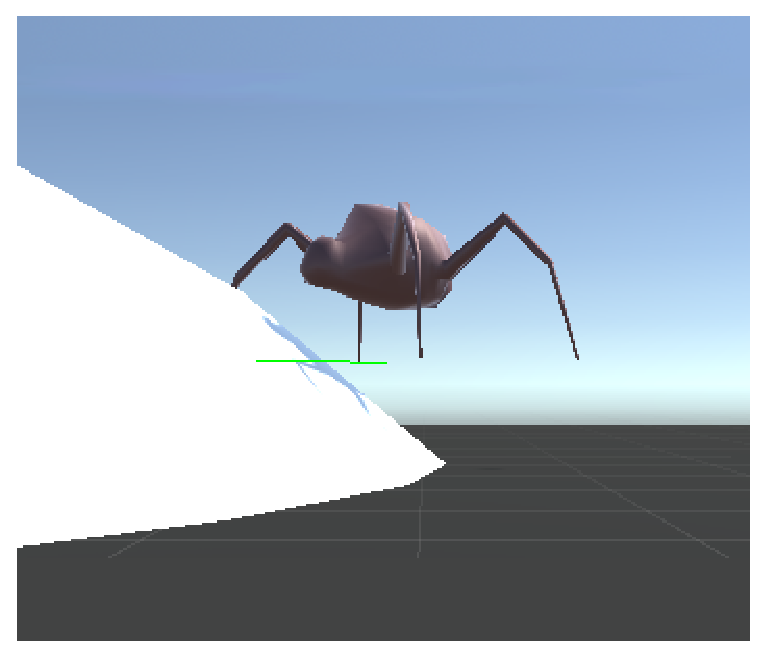
\includegraphics[width=0.4\linewidth]{grafika/sp_b_round.eps}
        \hspace{0.1cm}
        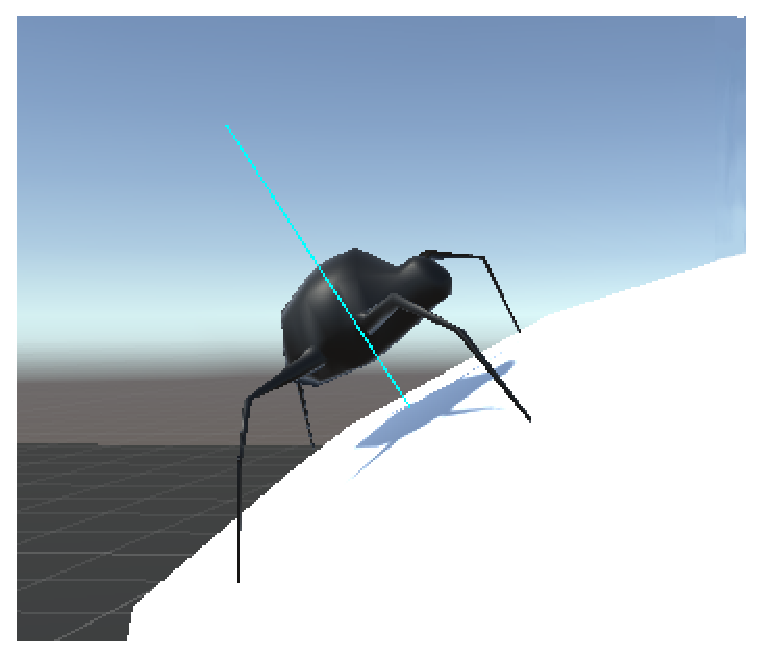
\includegraphics[width=0.4\linewidth]{grafika/sp_ik_round.eps}
        \subcaption{}
        \label{fig:sp_round}
    \end{subfigure}
    \begin{subfigure}{\textwidth}
        \centering
        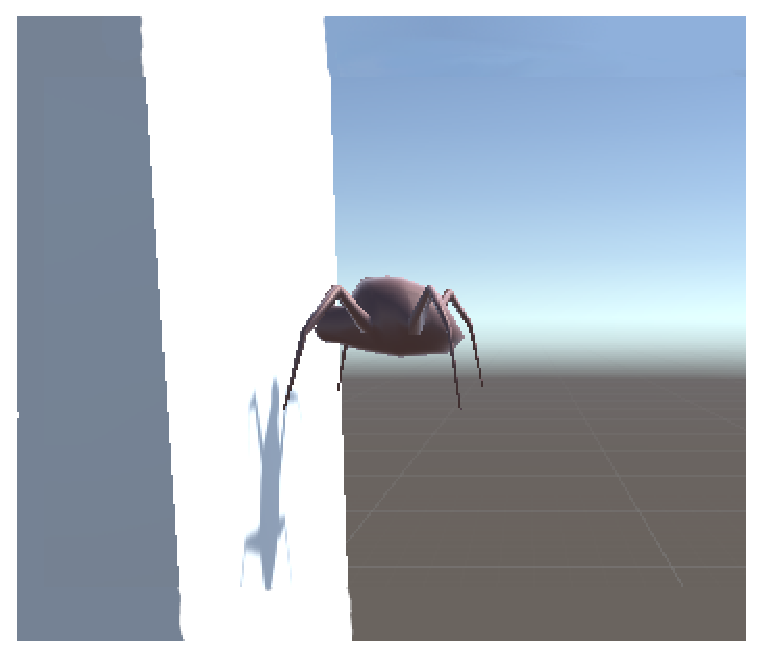
\includegraphics[width=0.4\linewidth]{grafika/sp_b_wall.eps}
        \hspace{0.1cm}
        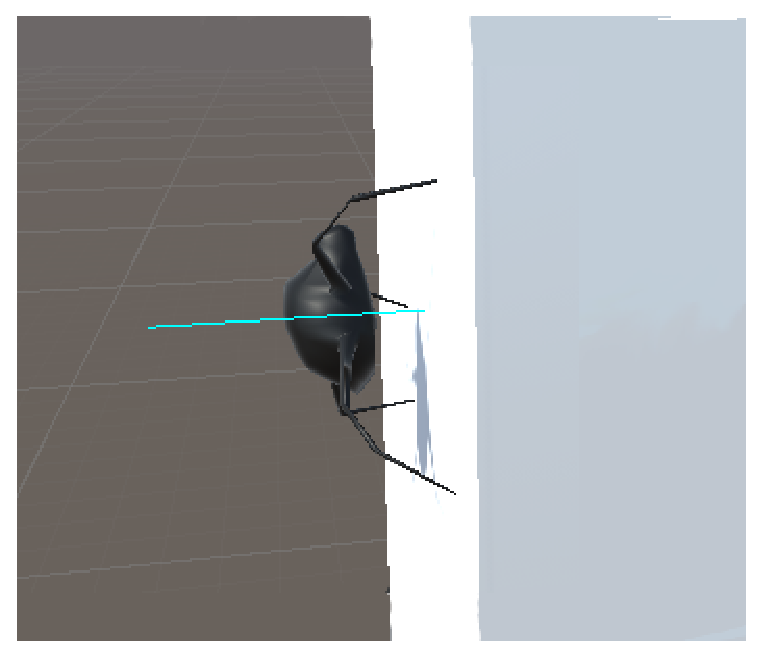
\includegraphics[width=0.4\linewidth]{grafika/sp_ik_wall.eps}
        \subcaption{}
        \label{fig:sp_wall}
    \end{subfigure}
    \caption{A comparison between the baked animation model (left) and IK
    model (right) of the spider.}
    \label{fig:spider_comparison}
\end{figure}


One important aspect to note when comparing the realism of both animations is
how the legs move relative to the surface on which they stand. In the case of
the procedural animation, the IK targets controlling the spider's legs remain
fixed in one place until a leg movement is initiated. As a result, no matter the
speed at which the spider is moving, the give the impression that they are
placed on the floor and push away realistically. On the contrary, the baked
animation is played at a certain speed, and it is very hard to match the
animation speed to the spider's movement speed so that the legs seem to stay in a fixed
position on the ground while the spider is moving. This breaks the illusion of
the legs pushing the spider forwards, as they instead glide on the surface out
of sync.

In certain games, the accuracy of animation sequences creates a greater
immersion for the player. In the event that the sequence of pressed buttons is
important, such as a player needing to provide a specific input to hack a code
to open a door, the realism of the game can be elevated through the use of
inverse kinematics. The adaptability of a character's actions can be seen in this
comparison between the baked and IK versions of the button press animation.

When the character is only required to press a single button, while also having
a proper position and orientation relative to the button, the baked animation
looks quite natural, and looks no different from the IK version as shown in Fig.
\ref{fig:h_single}.


The difference starts to be noticeable when the character is offset or rotated
from the default position. While the IK target leads the hand correctly to the
button, the baked animation has no knowledge of the characters surroundings, and
misses its mark (Fig. \ref{fig:h_offset}). Due to this, for realism to be
preserved when using a baked animation, either the character must be reoriented
as part of the action, or a cutscene should be played for the duration of the
action. 


\begin{figure}
    \centering
    \captionsetup{justification=centering}
    \begin{subfigure}{\textwidth}
        \centering
        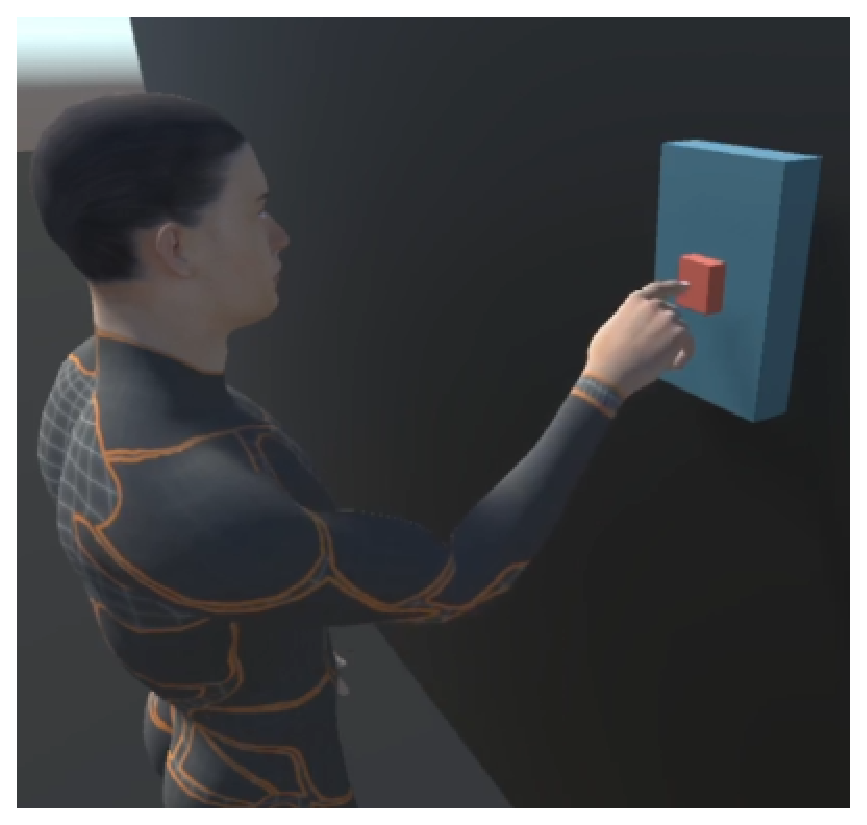
\includegraphics[width=0.4\linewidth]{grafika/h_b_single.eps}
        \hspace{0.1cm}
        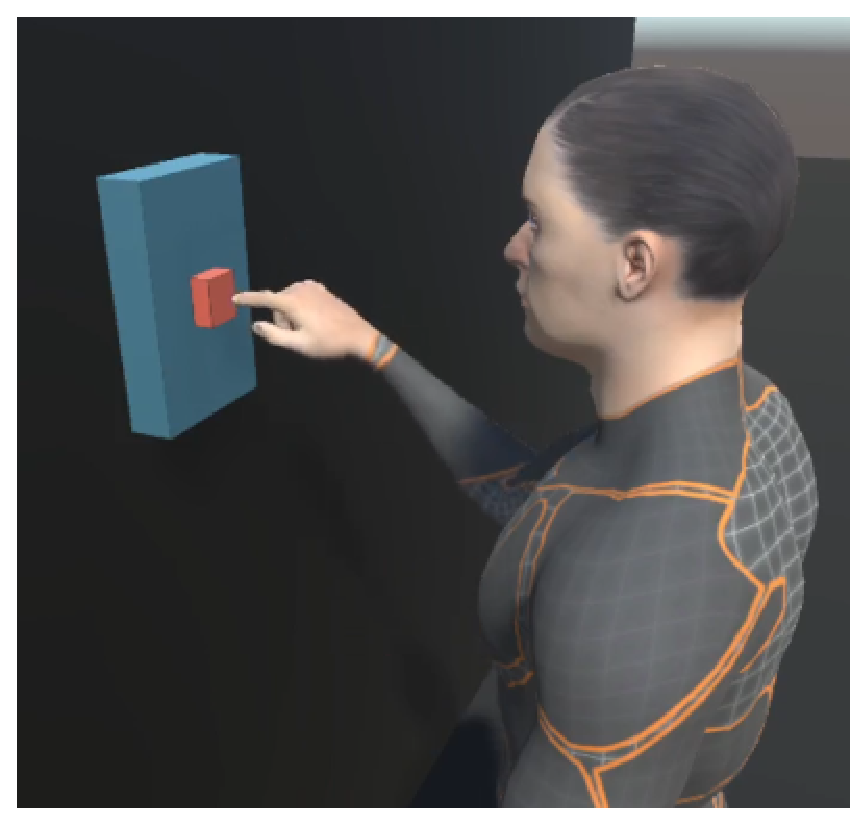
\includegraphics[width=0.4\linewidth]{grafika/h_ik_single.eps}
        \subcaption{}
        \label{fig:h_single}
    \end{subfigure}
    \begin{subfigure}{\textwidth}
        \centering
        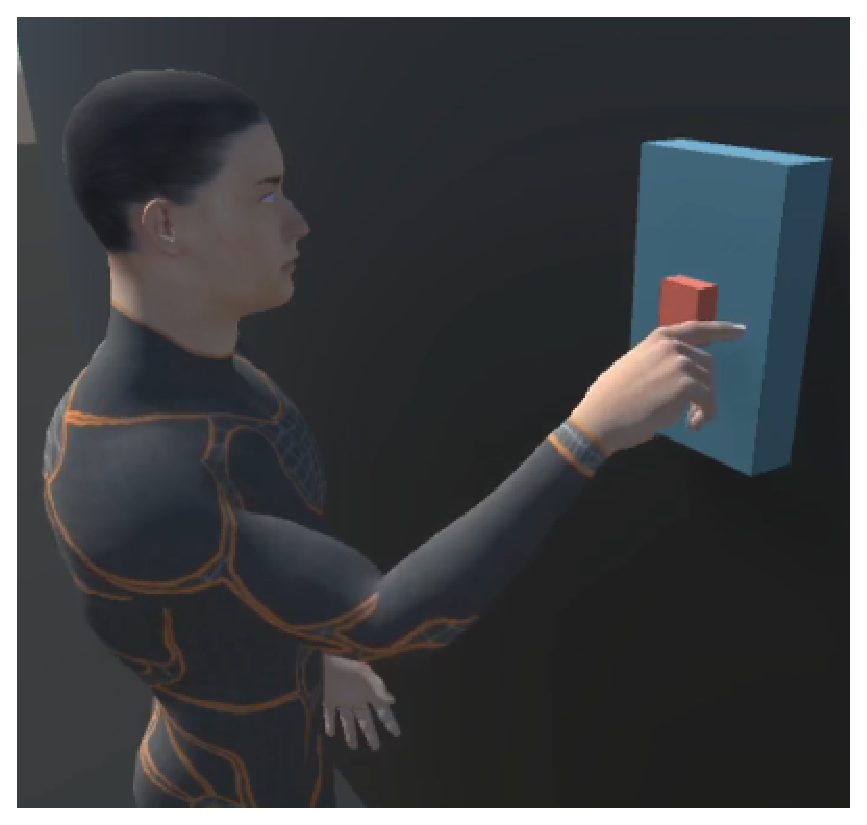
\includegraphics[width=0.4\linewidth]{grafika/h_b_offset.eps}
        \hspace{0.1cm}
        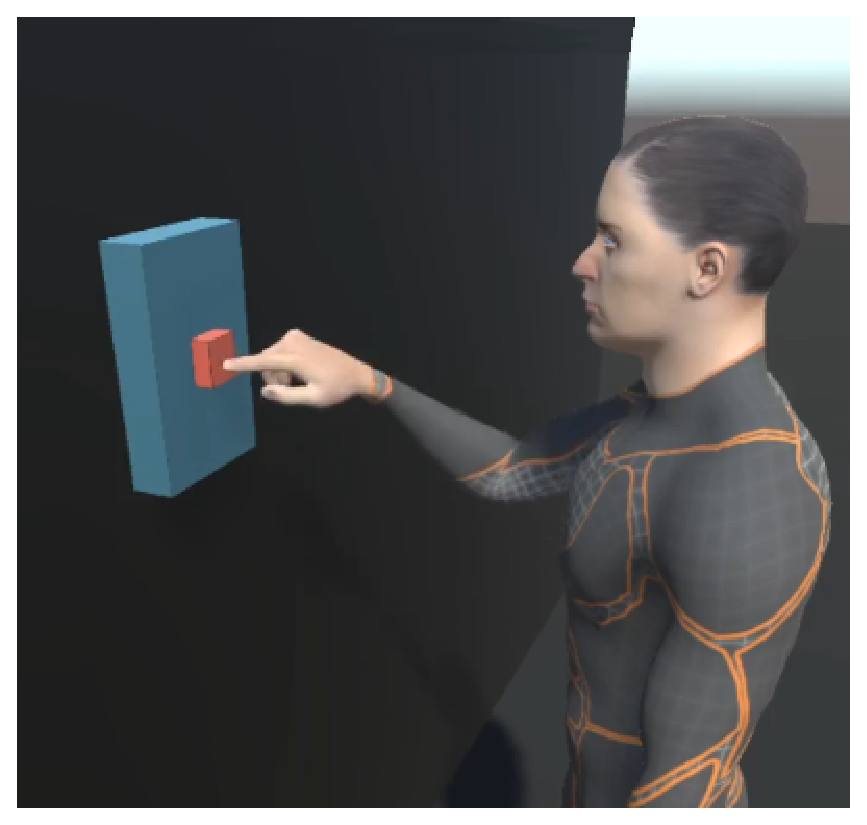
\includegraphics[width=0.4\linewidth]{grafika/h_ik_offset.eps}
        \subcaption{}
        \label{fig:h_offset}
    \end{subfigure}
    \caption{A comparison between the baked animation model (left) and IK model
    (right) of the human character. (a) shows both models executing the button
    press animation while being positioned and oriented correctly. (b) shows the
    models being offset and rotated from the default positioning.}
    \label{fig:human_comparison}
\end{figure}


The next benefit of the procedural animation is its ability to adapt to a panel
with multiple buttons. The character which is using the baked animation is only
able to aim its hand at one specific point, consequently missing all the
buttons. In the case of a sequence of buttons being pressed, the character
repeats the press in a single spot which doesn't realistically convey the
pressing of a sequence of buttons. This can be slightly improved by constructing
the animation to aim at different buttons on the panel in a generic order. The
downside of this approach is that it falls apart if there is a change in the
amount of buttons, or their positions and configuration. 

Comparing this to the IK animation, as seen in Fig. \ref{fig:h_ik_multiple},
the IK target leads the hand to the appropriate position for each separate
button. This allows for a specific sequence of buttons - taking the door hacking
example from before this would be a player's input - to be pressed in a way
which visually conveys the exact action which was commanded, in a responsive
manner.

\begin{figure}[h!]
    \centering
    \captionsetup{justification=centering}
    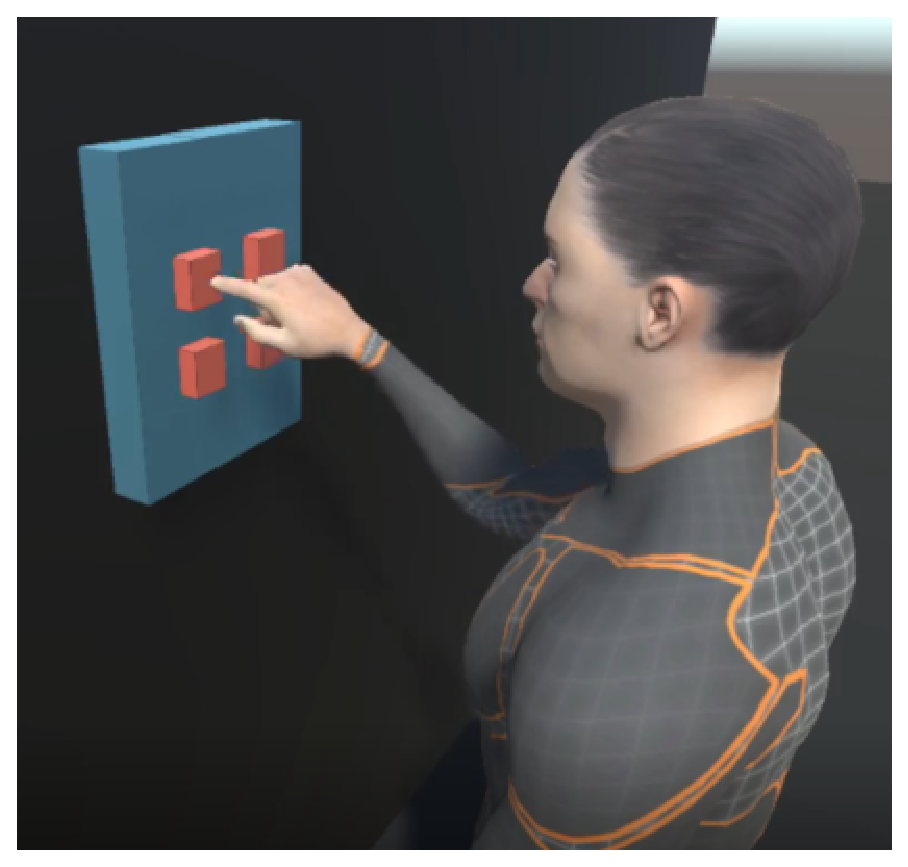
\includegraphics[width=0.4\textwidth]{grafika/h_ik_1.eps}
        \hspace{0.1cm}
    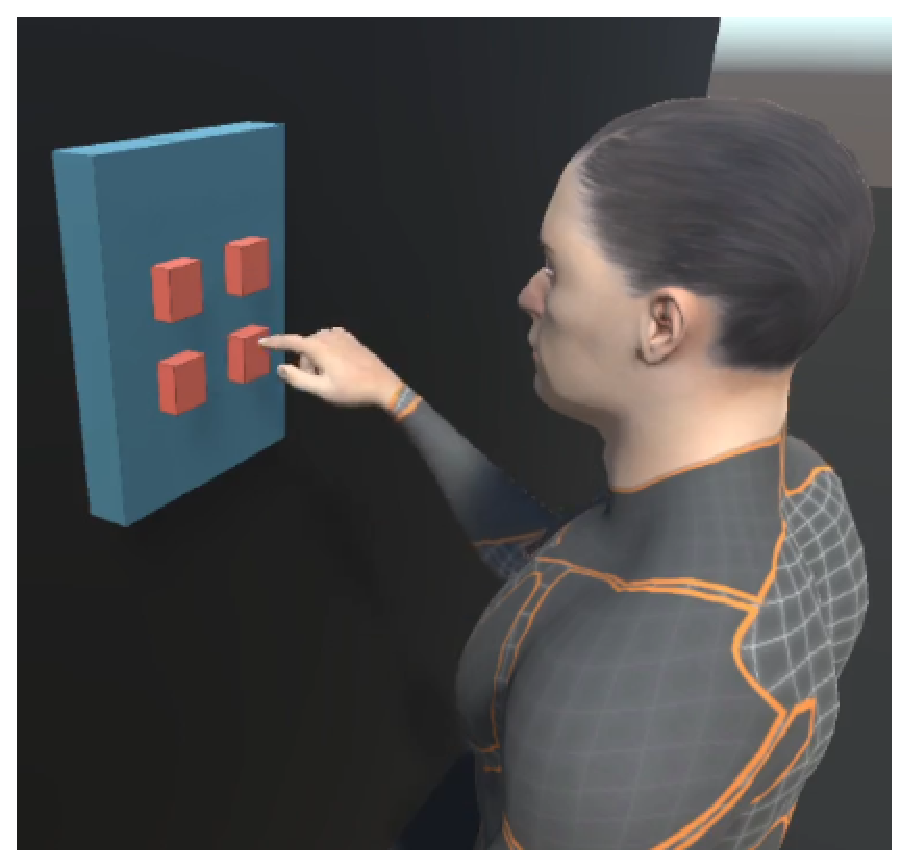
\includegraphics[width=0.4\textwidth]{grafika/h_ik_2.eps}

    \vspace{0.2cm}
    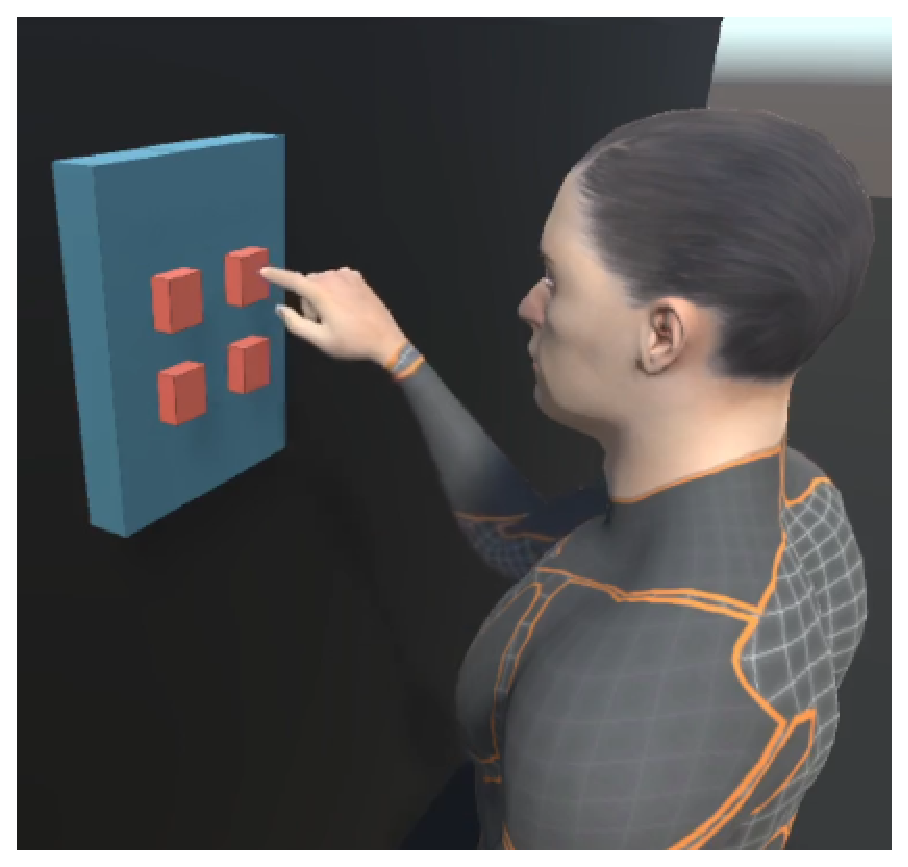
\includegraphics[width=0.4\textwidth]{grafika/h_ik_3.eps}
        \hspace{0.1cm}
    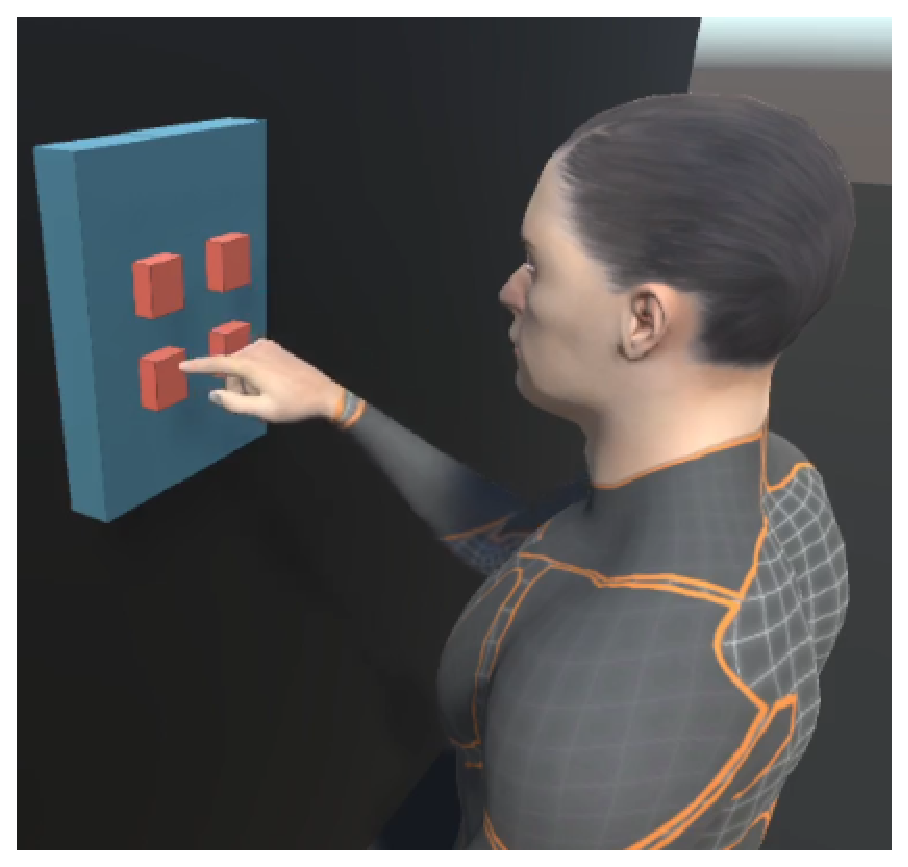
\includegraphics[width=0.4\textwidth]{grafika/h_ik_4.eps}
    \caption{The IK model pressing each of the four buttons on a panel}
    \label{fig:h_ik_multiple}
\end{figure}



\section{Performance Comparison}
One thing to consider when implementing a task procedurally is the
effect it may have on the performance of the application. Resorting to the use
of code and calculations instead of executing a predefined sequence introduces
the potential of increasing the CPU usage and decreasing performance. An
analysis was conducted on the examples created in the demo application using the
Unity Profiler \cite{unity_profiler}. Each experiment was carried out by
spawning 100 objects of each type and comparing the CPU usages both while they
were idle and while they were moving. Some usage categories were discarded as
they were not relevant to the analysis.

% \begin{figure}[h!]
%     \centering
%     \captionsetup{justification=centering}
%     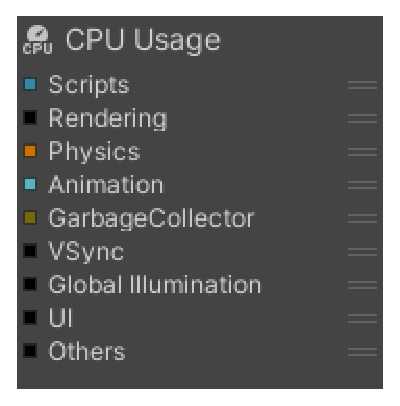
\includegraphics[width=0.5\textwidth]{grafika/profiler_settings.eps}
%     \caption{Usage categories selected when analyzing CPU usage}
%     \label{fig:profiler_settings}
% \end{figure}

Starting with the baked version of the spider, a hundred duplicates spawned
simultaneously produced the result seen in Fig. \ref{fig:pr_sp_b}. Similarly
to the IK version presented further down, most of the CPU usage comes from the
"scripts" usage category. A clear distinction can be made between when the
spider was moving and when it was not. During the profiling, the state of the
spider started out as idle, and then alternated between moving and idle at
approximately each quarter of the graph presented. In the idle state, the CPU
usage for the selected categories remains steadily below 10 milliseconds.
However, when the spider is moving the usage rises with an initial spike which
is almost double that of the idle state, and then lowering to around 10
milliseconds. The increase in CPU usage, as seen from the profiler, is mostly in
the "scripts" category, which means that the animations themselves are not
influencing the performance of the application too much.

The IK version of the spider has a much more steady average regardless of its
moving or idle state. In Fig. \ref{fig:pr_sp_ik}, the graph rises minimally at the
halfway mark which is where the spiders were transitioned to a moving state.
The lack of distinct change between states can be attributed to the fact that
the IK calculations done on the kinematic chains and their respective targets
are done regardless if the spider is moving or not. The same can be said for the
raycasts and body rotation calculations which are executed no matter the state.
The slight increase is most likely due to the calculations required to determine
the forward movement vector when the spider receives input. 

\begin{figure}
    \centering
    \captionsetup{justification=centering}
    \begin{subfigure}{\textwidth}
        \centering
        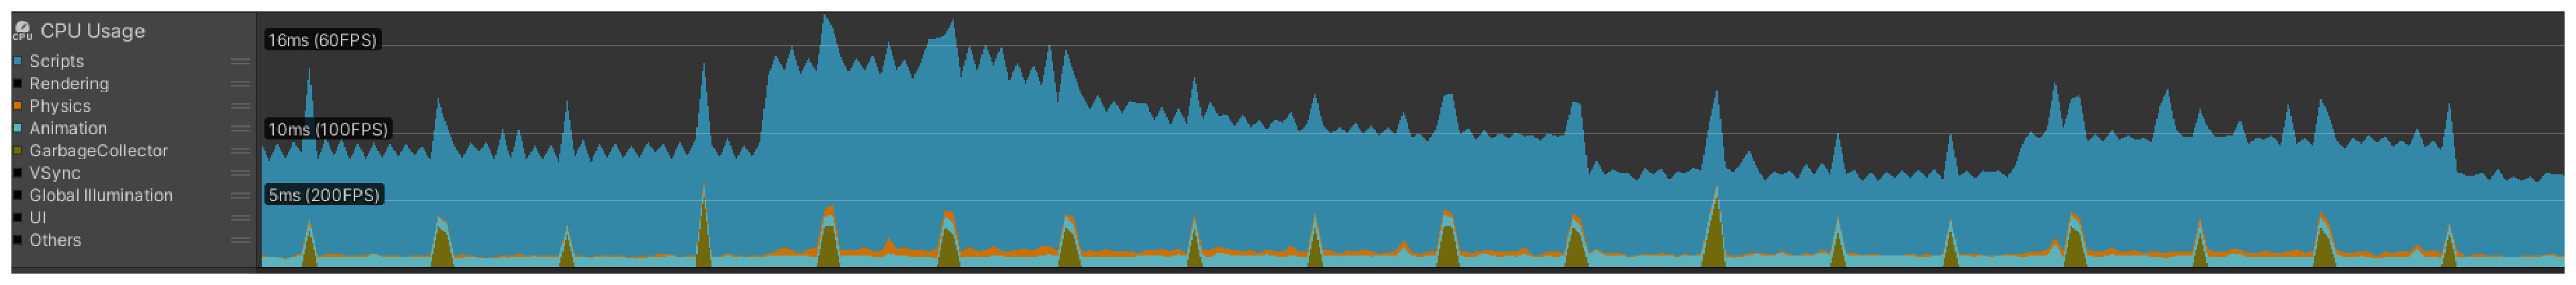
\includegraphics[width=\linewidth]{grafika/pr_sp_b.eps}
        \subcaption{}
        \label{fig:pr_sp_b}
    \end{subfigure}
    \begin{subfigure}{\textwidth}
        \centering
        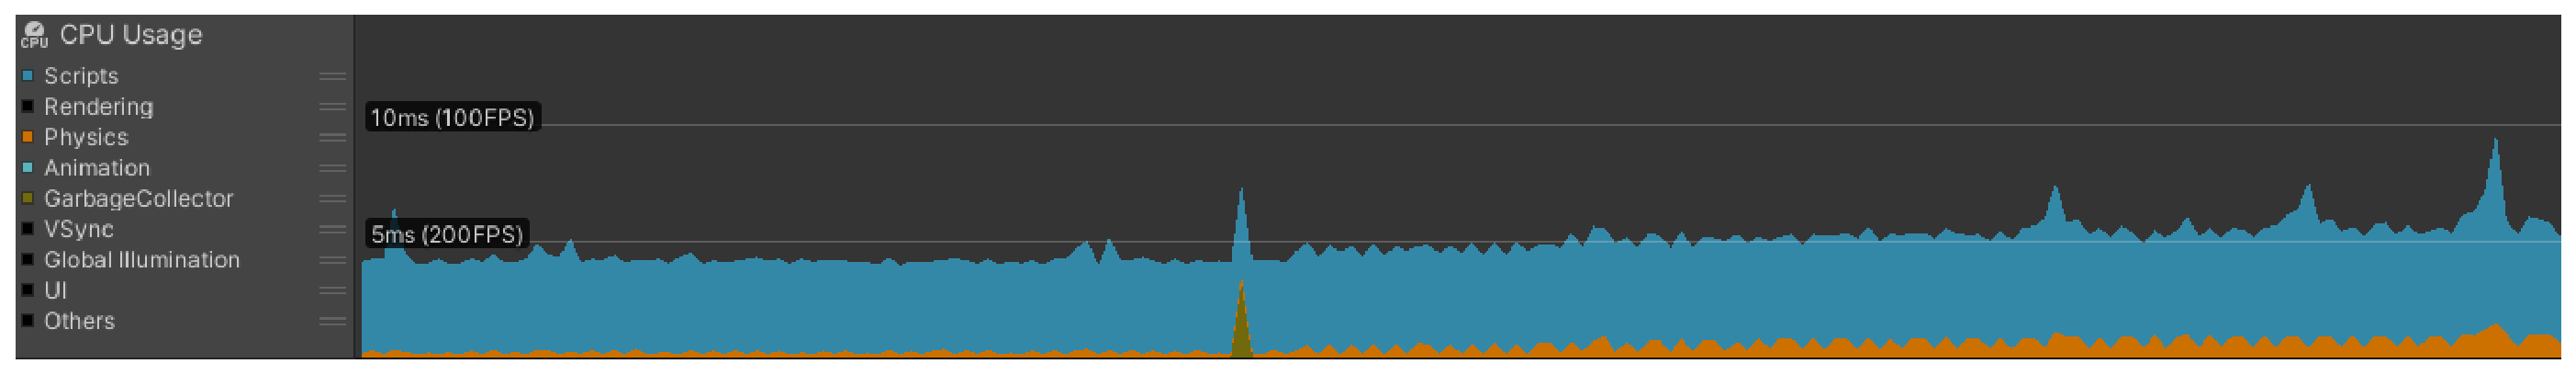
\includegraphics[width=\linewidth]{grafika/pr_sp_ik.eps}
        \subcaption{}
        \label{fig:pr_sp_ik}
    \end{subfigure}
    \caption{A comparison between the CPU usage profiling of one hundred
    instances of the spider baked animations (a) and with procedural IK
    animations (b).}
    \label{fig:pr_sp}
\end{figure}

The average CPU usage for the IK version of the spider is around half that of its
baked counterpart. This is most likely due to the baked animation spider
requiring more checks and calculations which pertain to the physics of its
movement. The IK version does not need many physics checks as the simple ray
cast system keeps the spider stuck to the surface, and combined with the IK
mechanism it moves the spider along without the need for collision checking.
However, this is relevant for the implementation presented in this demo
application, and may not be the case if a given use case required the spider to
be able to register collisions and be affected by gravity.

The purpose of the human character in the demo application is to demonstrate
a specific animation sequence executed through the means of baked and procedural
animations. Because there are no collisions, movement, or other checks, the baked
animation character's script contains almost no major calculations. Since
baked animations do not have a big influence on the CPU usage as seen earlier in
the case of the spider, the performance of the application does not vary in
relation to when the button pressing sequence is executed. Fig.
\ref{fig:pr_h_b} displays the results of profiling one hundred instances of the
baked animation human characters executing the animation sequence
simultaneously, and no spike in CPU usage, which hovers around 1ms, can be
observed

In contrast, the procedurally animated human does require a few calculations
during the animations sequence. While it does use baked animations for the
beginning and end of the sequence, the middle section switches to using inverse
kinematics, and additionally the IK targets are interpolated between the hand's
origin position and the button target positions. These calculations can be
seen in Fig. \ref{fig:pr_h_ik} where during the execution of the animation
there is a noticeable spike in the "scripts" usage category. Other than that,
the rest of the graph looks very similar to the baked animation variant, sitting
at around 1 milliseconds of CPU usage.

\begin{figure}
    \centering
    \captionsetup{justification=centering}
    \begin{subfigure}{\textwidth}
        \centering
        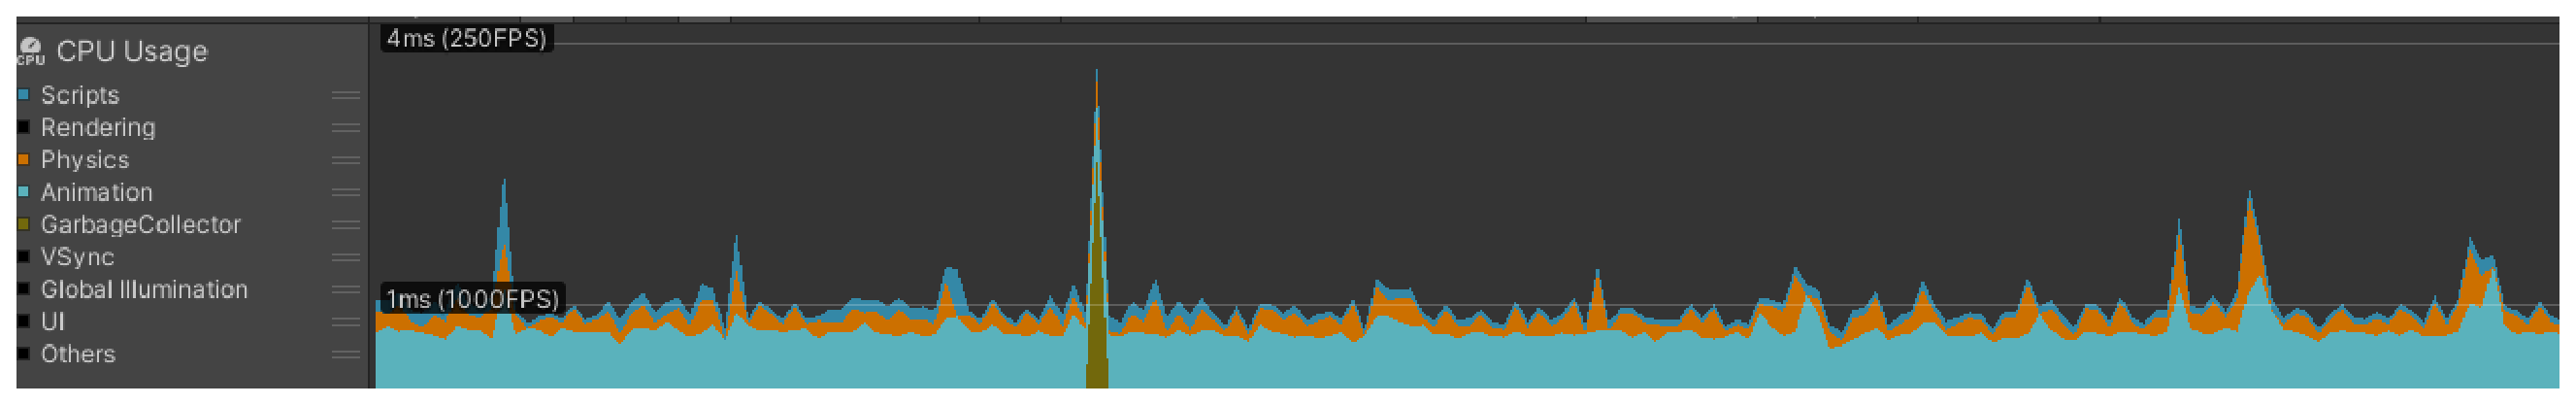
\includegraphics[width=\linewidth]{grafika/pr_h_b.eps}
        \subcaption{}
        \label{fig:pr_h_b}
    \end{subfigure}
    \begin{subfigure}{\textwidth}
        \centering
        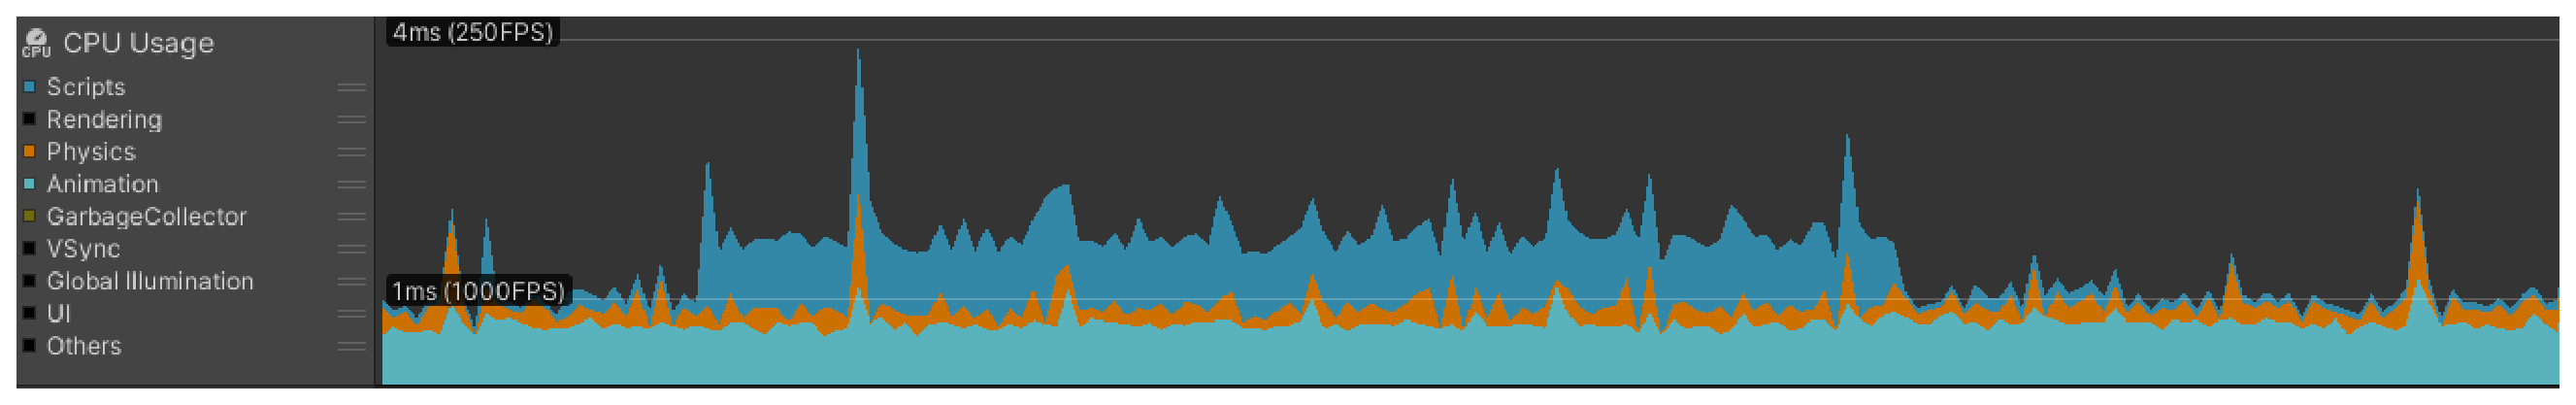
\includegraphics[width=\linewidth]{grafika/pr_h_ik.eps}
        \subcaption{}
        \label{fig:pr_h_ik}
    \end{subfigure}
    \caption{A comparison between the CPU usage profiling of one hundred
    instances of the human character with baked animations (a) and with
    procedural IK animations (b).}
    \label{fig:pr_h}
\end{figure}

